\documentclass[t, utf8x, 10pt]{beamer}
\usepackage[ngerman]{babel}
\usepackage{bera}
\usepackage{fontawesome}
\usepackage{listings}
\usepackage{url}

\setbeamertemplate{navigation symbols}{}

\hypersetup{%
  pdftitle={Pythonskripte testen: wie und warum?}
  ,pdfauthor={Gert-Ludwig Ingold <gert.ingold@physik.uni-augsburg.de>}
  ,pdfsubject={Linux Infotag 2016, Augsburg, 16.4.2016}
  ,pdfkeywords={Python, testing, doctests, unittests}
}

\graphicspath{{./img/}}

\definecolor{c1}{hsb}{0.125, 1, 0.8}
\definecolor{c2}{hsb}{0.458, 1, 0.6}
\definecolor{c3}{hsb}{0.791, 1, 0.8}
\definecolor{pro}{rgb}{0, 0.6, 0}
\definecolor{contra}{rgb}{0.8, 0, 0}

\lstset{language=Python,
        basicstyle={\ttfamily},
        showstringspaces=false,
        keywordstyle=\color{c2},
        commentstyle=\color{c3},
        stringstyle=\color{c1}
        }

\newcommand\pro{\textcolor{pro}{\faicon{smile-o}}}
\newcommand\contra{\textcolor{contra}{\faicon{frown-o}}}


\begin{document}

\begin{frame}[fragile]
 \vspace{1truecm}
 \begin{center}
  \structure{\LARGE Pythonskripte testen: wie und warum?}\\[0.3truecm]
  {\large Gert-Ludwig Ingold}

  \vspace{0.5truecm}
  \begin{minipage}{0.5\textwidth}
   \begin{tiny}
    \begin{lstlisting}[backgroundcolor=\color{black!10}
                       ,language={}]
 **********************************************
 File "example", line 1, in example
 Failed example:
     1+1
 Expected:
     1
 Got:
     2
 **********************************************
 1 items had failures:
     1 of   1 in example
 ***Test Failed*** 1 failures.
    \end{lstlisting}
   \end{tiny}
  \end{minipage}

  \vspace{1truecm}
  \faicon{github}
  \texttt{\normalsize git clone https://github.com/gertingold/lit2016.git}
 \end{center}
\end{frame}


\begin{frame}[c]{Wer testet seine Programme?}
 \begin{itemize}
  \item[\pro]    Programme werden praktisch immer bei der Programmentwicklung
	         durch Vergleich mit dem erwarteten Verhalten getestet.
  \item[\contra] Das passiert oft sehr informell und kaum reproduzierbar.
 \end{itemize}

 \uncover<2>{%
 erster Bug (1947):
 \begin{center}
  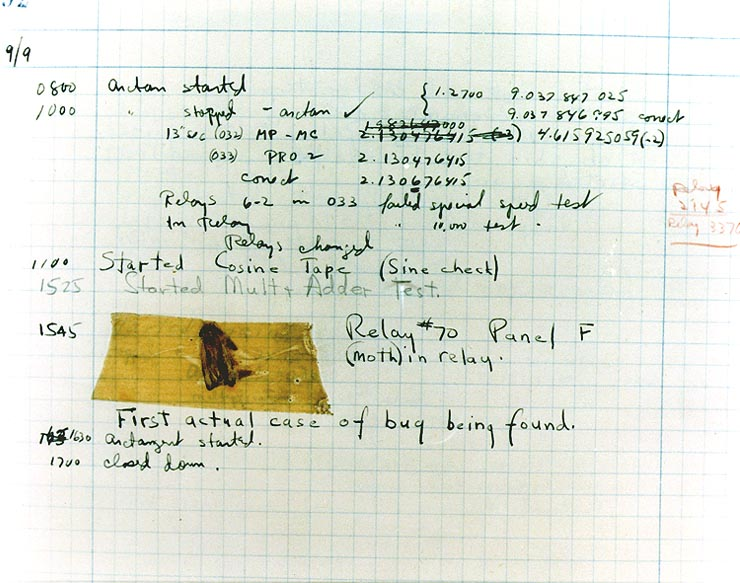
\includegraphics[width=0.6\textwidth]{H96566k.jpg}
 \end{center}}
\end{frame}


\begin{frame}[fragile]{Einige Überlegungen zum Testen}
 \begin{itemize}
  \item Tests dokumentieren überprüfte Funktionalität von Code\\[0.2truecm]
	  Beispiel: \parbox[t]{0.7\textwidth}{\url{https://hg.python.org/cpython/file/tip/Lib/test/test\_math.py}}
    \begin{lstlisting}
    ...
    def testSqrt(self):
	self.assertRaises(TypeError, math.sqrt)
        self.ftest('sqrt(0)', math.sqrt(0), 0)
        self.ftest('sqrt(1)', math.sqrt(1), 1)
        self.ftest('sqrt(4)', math.sqrt(4), 2)
        self.assertEqual(math.sqrt(INF), INF)
        self.assertRaises(ValueError, math.sqrt, NINF)
        self.assertTrue(math.isnan(math.sqrt(NAN)))
    ...
    \end{lstlisting}
 \end{itemize}
\end{frame}


\begin{frame}[fragile]{Einige Überlegungen zum Testen}
 \begin{itemize}
  \item Tests dokumentieren überprüfte Funktionalität von Code
  \item Tests sollten jederzeit erlauben, rasch die Funktionalität des Codes zu überprüfen
	\begin{itemize}
         \item vor dem Einchecken ins Versionskontrollsystem
	 \item beim Refactoring
	 \item \dots
	\end{itemize}
  \item Testsuites sind (praktisch) nie vollständig
	\begin{itemize}
	 \item zu jedem gefundenen Fehler einen Test schreiben, damit der Fehler nie
	       wieder auftreten kann
	 \item zu jedem neuen Feature Tests schreiben
         \item ggf. immer wieder Tests ergänzen
	\end{itemize}
  \item Tests sollten den Code (nahezu) vollständig ausführen\\
        siehe \texttt{coverage.py} (\url{coverage.readthedocs.org})
  \item gut getester Code, z.B. aus der Python Standard Library, muss nicht noch einmal
        getestet werden
 \end{itemize}
\end{frame}


\begin{frame}[c]{Unittests}
 \begin{itemize}
  \item \structure{Unittest}: \parbox[t]{0.78\textwidth}{Test von elementaren Einheiten
	  eines Programms, z.B. Funktionen oder Methoden}\\[0.2truecm]
  \item Unittests erleichtern die Lokalisierung von Fehlern
  \item Unittests unterstützen eine modularisierte Programmierweise und verbessern
	damit den Code
  \item das Zusammenspiel von Komponenten muss separat getestet werden (Integrationstests,
	Systemtests)
  \item das \texttt{unittest}-Modul von Python kann auch für Integrationstests verwendet
	werden
 \end{itemize}
\end{frame}


\begin{frame}[c]
 \begin{Large}
  Zwei Module aus der Python Standard Library:
  \setbeamercovered{transparent=30}
  \begin{itemize}
   \item<1-2> \texttt{doctest}
   \item<1>   \texttt{unittest}
  \end{itemize}
  \setbeamercovered{invisible}
 \end{Large}
\end{frame}


\begin{frame}[fragile]{Was sind Docstrings?}
 \lstinputlisting{../examples/doctests/example1_v1.py}

 \hrulefill

 \structure{in der Python-Shell:}
 \begin{lstlisting}[language={}]
 >>> help(welcome)

 Help on function welcome in module __main__:

 welcome(name)
     be nice and greet somebody
     name: name of the person
 \end{lstlisting}
\end{frame}


\begin{frame}{Ein Gruß an Guido van Rossum}
 \lstinputlisting{../examples/doctests/example1_v2.py}

 \hrulefill
 \begin{itemize}
  \item die Benutzung der Funktion wird dokumentiert
  \item dabei wird die Syntax der Python-Shell verwendet\\
	\texttt{{>}{>}{>}} \quad Eingabe-Prompt\\
	\texttt{...} \quad Fortsetzungszeile
  \item nach der Ausgabe folgt eine Leerzeile oder der nächste Prompt
  \item \alert{es lässt sich aber auch die korrekte Funktionsweise testen}
 \end{itemize}
\end{frame}


\begin{frame}[fragile]{Ein erster Test}
 Die Funktion sei in der Datei \texttt{example1\_v2.py} definiert:

 \begin{lstlisting}[language=bash]
 $ python -m doctest example1_v2.py
 $ 
 \end{lstlisting}

 \begin{itemize}
  \item »keine Neuigkeiten sind gute Neuigkeiten«\\
	oder:\\
	erfolgt keine Ausgabe, so wurden alle vorhandenen Tests fehlerfrei
	ausgeführt, sofern sie nicht unterdrückt wurden
  \item es wird das Modul \texttt{doctest} aus der Python-Standardbibliothek
	verwendet\\
	ausführliche Dokumentation unter:
	\url{http://docs.python.org/library/doctest.html}
  \item mit der Option \texttt{-v} wird \texttt{doctest} gesprächiger
 \end{itemize}
\end{frame}


\begin{frame}[fragile]{Und noch einmal mit mehr Details}
	\begin{lstlisting}[language={}]
 $ python -m doctest -v example1_v2.py
 Trying:
     welcome('Guido')
 Expecting:
     'Hallo Guido!'
 ok
 1 items had no tests:
     example1_v2
 1 items passed all tests:
     1 tests in example1_v2.welcome
 1 tests in 2 items.
 1 passed and 0 failed.
 Test passed.
 \end{lstlisting}
\end{frame}


\begin{frame}{Ein erster Fehler \dots}
 \lstinputlisting{../examples/doctests/example1_v3.py}
\end{frame}


\begin{frame}[fragile]{\dots und das Ergebnis}
 \begin{lstlisting}[language={}]
 $ python -m doctest example1_v3.py
 **********************************************************************
 File "example1_v3.py", line 6, in example1_v3.welcome
 Failed example:
     welcome('Guido')
 Expected:
     'Hello Guido!'
 Got:
     'Hallo Guido!'
 **********************************************************************
 1 items had failures:
    1 of   1 in example1_v3.welcome
 ***Test Failed*** 1 failures.
 \end{lstlisting}

 \begin{itemize}
  \item bei Fehlern werden Details auch ohne die Option \texttt{-v} ausgegeben
 \end{itemize}
\end{frame}


\begin{frame}[c]{Erst die Tests, dann das Programmieren}
 \begin{center}
  \begin{Large}
   \setlength\fboxsep{0.4truecm}	  
   \fbox{\parbox{0.85\textwidth}{\structure{Test-driven development (TDD):}\\
                                 Formuliere erst die Tests und entwickle dann das
                                 Programm bis alle Tests fehlerfrei ausgeführt werden.}
	}
  \end{Large}
 \end{center}
\end{frame}


\begin{frame}{Wunschliste als Tests}
 \lstinputlisting{../examples/doctests/example1_v4.py}
\end{frame}


\begin{frame}[fragile]{Fehler, die es zu beseitigen gilt}
 \begin{tiny}
	 \begin{lstlisting}[language={}]
 **********************************************************************
 File "example1_v4.py", line 6, in example1_v4.welcome
 Failed example:
     welcome()
 Exception raised:
     Traceback (most recent call last):
       File "python3.5/doctest.py", line 1320, in __run
	 compileflags, 1), test.globs)
       File "<doctest example1_v4.welcome[0]>", line 1, in <module>
         welcome()
     TypeError: welcome() missing 1 required positional argument: 'name'
 **********************************************************************
 File "example1_v4.py", line 9, in example1_v4.welcome
 Failed example:
     welcome(lang='de')
 Exception raised:
     Traceback (most recent call last):
       File "python3.5/doctest.py", line 1320, in __run
         compileflags, 1), test.globs)
       File "<doctest example1_v4.welcome[1]>", line 1, in <module>
         welcome(lang='de')
     TypeError: welcome() got an unexpected keyword argument 'lang'
 **********************************************************************
 File "example1_v4.py", line 12, in example1_v4.welcome
 Failed example:
     welcome('Guido')
 Expected:
     'Hello Guido!'
 Got:
     'Hallo Guido!'
 **********************************************************************
 1 items had failures:
    3 of   3 in example1_v4.welcome
 ***Test Failed*** 3 failures.
  \end{lstlisting}
 \end{tiny}
\end{frame}


\begin{frame}{Ausnahmen sind manchmal gewollt}
 \begin{tiny}
  \lstinputlisting{../examples/doctests/example1_v5.py}
 \end{tiny}

 \begin{itemize}
  \item eine nicht implementierte Sprache soll zu einem \texttt{ValueError} führen
 \end{itemize}
\end{frame}


\begin{frame}[fragile]{Behandlung von Ausnahmen}
 \begin{itemize}
  \item Problem: die Ausgabe ist häufig komplex
 \end{itemize}
 \begin{footnotesize}
  \begin{lstlisting}[language={}]
 Traceback (most recent call last):
   File "example1_v6.py", line 25, in welcome
     greeting = greetings[lang]
 KeyError: 'nl'

 During handling of the above exception, another exception occurred:

 Traceback (most recent call last):
   File "example1_v6.py", line 33, in <module>
     welcome('Guido', 'nl')
   File "example1_v6.py", line 28, in welcome
     raise ValueError(errmsg)
 ValueError: unknown language: nl
  \end{lstlisting}
 \end{footnotesize}
 \begin{itemize}
  \item als Doctest genügt aber:
 \end{itemize}
 \begin{footnotesize}
 \lstinputlisting[linerange=16-18]{../examples/doctests/example1_v6.py}
 \end{footnotesize}
\end{frame}


\begin{frame}[fragile]{Direktiven für \texttt{doctest}}
 \begin{itemize}
  \item Platzhalter für beliebige Ausgabe
 \end{itemize}
 \begin{footnotesize}
  \lstinputlisting[linerange=16-18]{../examples/doctests/example1_v7.py}
 \end{footnotesize}

 \begin{itemize}
  \item der Test soll vorläufig nicht durchgeführt werden
 \end{itemize}
 \begin{footnotesize}
  \lstinputlisting[linerange=20-21]{../examples/doctests/example1_v7.py}
 \end{footnotesize}

 \begin{itemize}
  \item siehe die Dokumentation für weitere Direktiven:
	\url{http://docs.python.org/library/doctest.html}
  \item interessant ist z.B. noch \texttt{+NORMALIZE\_WHITESPACE}
 \end{itemize}
\end{frame}


\begin{frame}[fragile]{Doctests in beliebigem Text}
 Doctests sind nicht auf die Verwendung Docstrings begrenzt, sondern können in
 beliebige Textdateien eingebettet und dort getestet werden.

 \begin{columns}
  \begin{column}{0.5\textwidth}
   \texttt{example2.txt:}
   \begin{footnotesize}
    \lstinputlisting[language={}]{../examples/doctests/example2.txt}
   \end{footnotesize}
  \end{column}
  \begin{column}{0.5\textwidth}
   \begin{footnotesize}
    \begin{lstlisting}[language={}]
 $ python -m doctest -v example2.txt
 Trying:
     x = 1
 Expecting nothing
 ok
 Trying:
     if x < 0:
         print('x ist negativ')
     else:
         print('x ist nicht negativ')
 Expecting:
     x ist nicht negativ
 ok
 1 items passed all tests:
    2 tests in example2.txt
 2 tests in 1 items.
 2 passed and 0 failed.
 Test passed.
    \end{lstlisting}
   \end{footnotesize}
  \end{column}
 \end{columns}
\end{frame}


\begin{frame}[c]{Vor- und Nachteile von Doctests}
 \begin{itemize}
  \item[\pro]    leicht zu schreiben
  \item[\pro]    unterstützt die Dokumentation durch Beschreibung des
	         Benutzerinterfaces
  \item[\pro]    lässt sich -- im Gegensatz zum Rest der Dokumentation -- leicht
	         auf Korrektheit überprüfen
  \item[\pro]    kann zum Testen von Code in jeder Art von Text verwendet
                 werden\\[0.5truecm]
  \item[\contra] nicht gut für aufwändigere Testsuiten geeignet, zumindest nicht
	         in Docstrings
  \item[\contra] nicht für alle Testszenarien geeignet, z.B. Tests
	         von numerischen Codes bei denen das Ergebnis typischerweise
		 nur näherungsweise korrekt ist
 \end{itemize}
\end{frame}


\begin{frame}[c]
 \begin{Large}
  Zwei Module aus der Python Standard Library:
  \setbeamercovered{transparent=30}
  \begin{itemize}
   \item<1> \texttt{doctest}
   \item<1-2>   \texttt{unittest}
  \end{itemize}
  \setbeamercovered{invisible}
 \end{Large}
\end{frame}


\begin{frame}[fragile]{Pascalsches Dreieck}
 \begin{small}
  \lstinputlisting{../examples/unittests/pascal_v1.py}

  \begin{lstlisting}[language={}]
 $ python pascal_v1.py 
 0             1           
 1           1  1          
 2          1  2  1        
 3        1  3  3  1       
 4       1  4  6  4  1     
 5     1  5 10 10  5  1    
 6    1  6 15 20 15  6  1 
  \end{lstlisting}
 \end{small}
\end{frame}


\begin{frame}[fragile]{Erste Unittests}
 \texttt{test\_pascal\_v1.py:}
 \begin{scriptsize}
  \lstinputlisting{../examples/unittests/test_pascal_v1.py}

  \hrulefill

  \begin{lstlisting}[language={}]
 $ python test_pascal_v1.py 
 ...
 ----------------------------------------------------------------------
 Ran 3 tests in 0.000s
 
 OK
  \end{lstlisting}
 \end{scriptsize}
 \begin{itemize}
	 \item die Namen von Test-Methoden müssen mit \texttt{test} beginnen
 \end{itemize}
\end{frame}


\begin{frame}{Ein Fehler ...}
 \texttt{test\_pascal\_v2.py:}
 \begin{small}
  \lstinputlisting{../examples/unittests/test_pascal_v2.py}
 \end{small}
 \begin{itemize}
  \item Der Fehler wurde hier in den Test eingebaut, er könnte aber genauso
        gut im Programm stecken.
 \end{itemize}
\end{frame}


\begin{frame}[fragile]{... und das Ergebnis}
 \begin{scriptsize}
  \begin{lstlisting}[language={}]
 $ python test_pascal_v2.py
 ..F
 ======================================================================
 FAIL: test_n5 (__main__.TestExplicit)
 ----------------------------------------------------------------------
 Traceback (most recent call last):
   File "test_pascal_v2.py", line 12, in test_n5
     self.assertEqual(list(pascal(5)), [1, 4, 6, 4, 1])
 AssertionError: Lists differ: [1, 5, 10, 10, 5, 1] != [1, 4, 6, 4, 1]

 First differing element 1:
 5
 4

 First list contains 1 additional elements.
 First extra element 5:
 1

 - [1, 5, 10, 10, 5, 1]
 + [1, 4, 6, 4, 1]

 ----------------------------------------------------------------------
 Ran 3 tests in 0.001s

 FAILED (failures=1)
  \end{lstlisting}
 \end{scriptsize}
\end{frame}


\begin{frame}[fragile]{Ein erwarteter Fehler}
 Auszug aus \texttt{test\_pascal\_v3.py:}
 \begin{small}
 \lstinputlisting[linerange=1-1]{../examples/unittests/test_pascal_v3.py}
 [...]
 \lstinputlisting[linerange=4-4]{../examples/unittests/test_pascal_v3.py}
 [...]
 \lstinputlisting[linerange=11-13]{../examples/unittests/test_pascal_v3.py}

 \hrulefill

  \begin{lstlisting}[language={}]
 $ python test_pascal_v3.py
 ..x
 ------------------------------------------------------------------
 Ran 3 tests in 0.001s

 OK (expected failures=1)
  \end{lstlisting}
 \end{small}
\end{frame}


\begin{frame}{Was tun bei größeren Argumenten?}
bei großen Argumenten ist es nicht mehr sinnvoll, gegen das explizite Resultat
zu testen $\rightarrow$ andersartige Tests sind erforderlich

\vspace{\baselineskip}
binomische Formeln:
\begin{displaymath}
 \begin{aligned}
  (a+b)^2 &= 1\cdot a^2+2\cdot ab+1\cdot b^2\\
  (a-b)^2 &= 1\cdot a^2-2\cdot ab+1\cdot b^2
 \end{aligned}
\end{displaymath}
Die Koeffizienten sind die Einträge bzw. die Einträge mit alternierendem Vorzeichen
aus dem pascalschen Dreieck für $n=2$.

\vspace{\baselineskip}
Für $a=b=1$:
\begin{displaymath}
 \begin{aligned}
  1+2+1 &= 2^2\hspace{0.2truecm} \text{allgemein:}\ 2^n \\
  1-2+1 &= 0\hspace{0.35truecm}    \text{gilt für alle $n$} \\
 \end{aligned}
\end{displaymath}

\vspace{1\baselineskip}
weitere Möglichkeit:

Überprüfe, ob sich aufeinanderfolgende Zeilen des pascalschen Dreiecks durch
Addition von benachbarten Elementen erzeugen lassen.
\end{frame}


\begin{frame}{Implementation der Tests (I)}
 \begin{small}
  [...]
  \lstinputlisting[linerange=15-22]{../examples/unittests/test_pascal_v4.py}
  [...]
  \lstinputlisting[linerange=33-37]{../examples/unittests/test_pascal_v4.py}
  [...]
 \end{small}
\end{frame}


\begin{frame}{Implementation der Tests (II)}
 \begin{small}
  \lstinputlisting[linerange=1-1]{../examples/unittests/test_pascal_v4.py}
  [...]
  \lstinputlisting[linerange=24-31]{../examples/unittests/test_pascal_v4.py}
  [...]
  \lstinputlisting[linerange=38-40]{../examples/unittests/test_pascal_v4.py}
  [...]
 \end{small}
\end{frame}


\begin{frame}{Testen auf Ausnahmen}
 Auszug aus \texttt{pascal\_v2.py}:
  \lstinputlisting[linerange=1-5]{../examples/unittests/pascal_v2.py}

 \vspace{\baselineskip}
 Auszug aus \texttt{test\_pascal\_v5.py}:
  \lstinputlisting[linerange=33-36]{../examples/unittests/test_pascal_v5.py}

 \begin{itemize}
  \item \texttt{assertRaises} kann auch außerhalb eines Kontexts benutzt werden,
	ist dann aber weniger übersichtlich
  \item der Generator beginnt erst mit der Ausführung des Codes, wenn ein
	Rückgabewert angefordert wurde
 \end{itemize}
\end{frame}


\begin{frame}{Erweiterung auf Floats}
 Unsere \texttt{pascal}-Methode kann leicht auf Float-Argumente angepasst werden.
 
 Beispiel:
 \begin{displaymath}
  \sqrt[3]{1+x} = 1+\frac{1}{3}x-\frac{1}{9}x^2+\frac{5}{81}x^3+\ldots
 \end{displaymath}

 \texttt{pascal\_v3.py:}
 \lstinputlisting{../examples/unittests/pascal_v3.py}

 Wenn $n$ keine nichtnegative ganze Zahl ist, gibt der Generator potentiell unendlich
 viele Werte zurück.
\end{frame}


\begin{frame}{Testen mit Floats}
 Auszug aus \texttt{test\_pascal\_v6.py}:
 \begin{small}
  \lstinputlisting[linerange=2-3]{../examples/unittests/test_pascal_v6.py}
  [...]
  \lstinputlisting[linerange=15-20]{../examples/unittests/test_pascal_v6.py}
  [...]
  \lstinputlisting[linerange=43-47]{../examples/unittests/test_pascal_v6.py}
 \end{small}
 \begin{itemize}
  \item unpassende Tests können mit dem \texttt{skip}-Dekorator deaktiviert werden
 \end{itemize}
\end{frame}


\begin{frame}[fragile]{Achtung, Rundungsfehler!}
 \begin{scriptsize}
  \begin{lstlisting}[language={}]
 $ python test_pascal_v6.py
 s...Fsss
 ======================================================================
 FAIL: test_one_third (__main__.TestFractional)
 ----------------------------------------------------------------------
 Traceback (most recent call last):
   File "test_pascal_v6.py", line 20, in test_one_third
     self.assertEqual(result, expected)
 AssertionError: Lists differ: [1, 0.3333333333333333, -0.11111111111111112,
 0.0617283950617284] != [1, 0.3333333333333333, -0.1111111111111111,
 0.06172839506172839]

 First differing element 2:
 -0.11111111111111112
 -0.1111111111111111

 - [1, 0.3333333333333333, -0.11111111111111112, 0.0617283950617284]
 ?                                            -                   ^

 + [1, 0.3333333333333333, -0.1111111111111111, 0.06172839506172839]
 ?                                                               ^^


 ----------------------------------------------------------------------
 Ran 8 tests in 0.001s

 FAILED (failures=1, skipped=4)
  \end{lstlisting}
 \end{scriptsize}
\end{frame}


\begin{frame}{Toleranz bei Floats}
 \begin{itemize}
  \item Verwendung von \texttt{math.isclose} (ab Python 3.5)
  \item \texttt{self.assertAlmostEqual}
  \item für Listen und NumPy-Arrays: \texttt{numpy.testing.assert\_allclose}\\
	damit lässt sich auch die Toleranz gut einstellen
 \end{itemize}

 Auszug aus \texttt{test\_pascal\_v7.py:}
 \lstinputlisting[linerange=3-3]{../examples/unittests/test_pascal_v7.py}
 [...]
 \lstinputlisting[linerange=16-21]{../examples/unittests/test_pascal_v7.py}

\end{frame}


\begin{frame}{Weiterführende Themen}
 \begin{itemize}
  \item \texttt{unittest}: Methoden \texttt{setUp} und \texttt{tearDown}, um
	vorbereitenden und abschließenden Code für Tests zu definieren
  \item \texttt{unittest.mock}: ersetzt benötigte Codeteile indem es eine
	definierte Funktionalität bereitstellt
  \item weitere Testwerkzeuge:\\
	\url{wiki.python.org/moin/PythonTestingToolsTaxonomy}\\
	z.B. \texttt{nose}, \texttt{coverage}
 \end{itemize}
\end{frame}

\end{document}
